%%%
%%% Cours de ``Programmation parallèle''. Polytech'Paris-UPMC
%%% par P. Fortin
%%% revisité et traduit en anglais par C. Bouillaguet

\documentclass{beamer}
\setbeamerfont{note page}{size=\tiny} % default = small 

\newcommand{\heading}{\frametitle}

\usecolortheme{rose}
\setbeamertemplate{footline}{}
\setbeamertemplate{navigation symbols}{}

\usepackage{amsmath, amssymb, amsthm}
\usepackage{epsfig}
\usepackage[utf8]{inputenc}
\usepackage[T1]{fontenc}
\usepackage[normalem]{ulem}   
\usepackage{framed}   
\usepackage{tabularx}
\usepackage{url}
\usepackage{psfrag}
\usepackage{alltt}
\usepackage{minted}
\definecolor{codebg}{rgb}{0.95,0.95,0.95}
\setminted{bgcolor=codebg}
\usepackage{changepage}

\newenvironment{wider}{%
\begin{adjustwidth}{-0.6cm}{}%
  \begin{minipage}{12cm}%
}{%
\end{minipage}%
\end{adjustwidth}%
}


\usepackage[formats]{listings}
\lstset{language=C, basicstyle=\scriptsize,showstringspaces=false,extendedchars=true}
\setminted{fontsize=\scriptsize}

\newcommand{\itemhappy}{\item[{\raisebox{-4pt}{
\includegraphics[height=12pt]{Content}}}]}
\newcommand{\itemsad}{\item[{\raisebox{-4pt}{
\includegraphics[height=12pt]{Triste}}}]}

\newtheorem{defi}{Définition}
\newtheorem{lemm}{Lemme}
\newtheorem{exem}{Exemple}
\newtheorem{theor}{Théorème}
\newtheorem{algo}{Algorithme}

\newcommand{\fixme}[1]{{\bf #1}}
\newcommand{\textstruct}[1]{{\color{beamerstructure} #1}}
\newcommand{\textstructbf}[1]{{\color{beamerstructure} \textbf{#1}}}

\newcommand{\mynote}[1]{\note<1>[item]{#1}}

\usepackage{fontspec}

\setsansfont{PalatinoSansLTPro}[
   Path = /home/charles/charles_work/fonts/PalatinoSans/, 
   Extension      = .otf,
   UprightFont    = *-Regular,
   BoldFont= *-Bold ,
   ItalicFont = *-Italic,
   BoldItalicFont = *-BoldIta
]


%\author[C.~Bouillaguet]{Charles Bouillaguet \newline
%  {\small \texttt{charles.bouillaguet@lip6.fr}}}

\title{Introduction to OpenMP}
%\date{2020-02-14}

\begin{document}


\begin{frame}
  \titlepage
\end{frame}
  
%%%%%%%%%%%%%%%%%%%%%%%%%%%%%%%%%%%%%%%%%%%%%%%%%%%%%%%%%%%%%%%%%%%%%%%

\begin{frame}
  \frametitle{Prologue: Thread VS Process}
  
  Process : ``control flow'' $~+~$ ``memory space'' \\
  Thread : ``control flow''
  
  \bigskip

  \begin{tabularx}{\textwidth}{X|X}
    Specific to each process & Specific to each thread \\
    \hline
    Memory (Heap)      & Instruction pointer  \\ 
    Global variables   & Registers \\
    Open Files         & Stack (local variables)\\
    child process, signals\dots & CPU state \\
  \end{tabularx}
  
  \bigskip

  \begin{tabularx}{\textwidth}{c|c}
    
\includegraphics[height=0.2\textheight]{multi-processus}$\quad$&
    
\includegraphics[height=0.2\textheight]{multi-thread}\\
    
    Multi-processes    &
    $\quad$ multi-threads $\quad$ \\
    
  \end{tabularx}
\end{frame}


%%%%%%%%%%%%%%%%%%%%%%%%%%%%%%%%%%%%%%%%%%%%%%%%%%%%%%%%%%%%%%%%%%%%%%%
\begin{frame}
  \frametitle{Prologue: Thread VS Process (continued)}

    \begin{columns}[t]
      \column{0.5\textwidth}
      \begin{center}
        Single-thread process:
        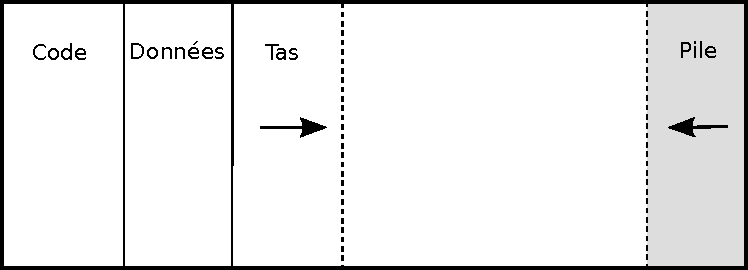
\includegraphics[height=0.2\textheight]{memoire_processus}
      \end{center}
      
      \column{0.5\textwidth}
      \begin{center}
        multi-thread process:
        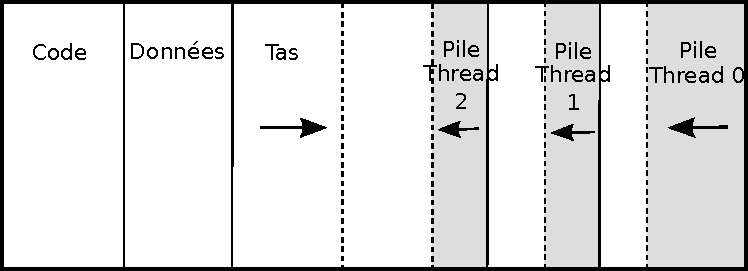
\includegraphics[height=0.2\textheight]{memoire_processus_multi-thread}
      \end{center}
    \end{columns}

    \bigskip 

    \begin{block}{All threads have access to the process' memory space}
      \begin{itemize}
        
      \item \textbf{\alert{Shared}} variables (between several threads)
        \begin{itemize}
        \item \emph{global} variables (``data segment'')
        \item Dynamically allocated variables with shared pointer
        \end{itemize}
        
        
      \item \textbf{\alert{private}} variables (``owned'' by a thread)
        \begin{itemize}
        \item Local variables (on the stack)
        \item Dynamically allocated variables with private pointer
        \end{itemize}
      \end{itemize}
    \end{block}
  \end{frame}

%%%%%%%%%%%%%%%%%%%%%%%%%%%%%%%%%%%%%%%%%%%%%%%%%%%%%%%%%%%%%%%%%%%%%%%%%



\begin{frame}
%  \heading{Avantages et inconvénients respectifs d'OpenMP / MPI }

  \begin{block}{OpenMP}
      \begin{itemize}
      \itemhappy Easier to use than MPI
      \itemhappy Preserve the original sequential code
      \itemhappy Code is easier to understand and maintain
      \itemhappy Allows progressive parallelization 
      \itemsad \alert{Shared memory} machines only (e.g. ONE server)
      \itemsad Works better on specific code patterns (loop nests, ...) 
      \end{itemize}
\end{block}

\begin{alertblock}{MPI}
      \begin{itemize}
      \itemhappy Designed for \textbf{distributed memory} machines
      \itemhappy Also works fine on shared-memory machines
      \itemhappy Separated memory spaces (no conflicts)
      \itemsad Algorithmic modifications often necessary
      \itemsad Harder to use
      \itemsad Performance depends on the network
      \end{itemize}
\end{alertblock}
  
  
\end{frame}



%%%%%%%%%%%%%%%%%%%%%%%%%%%%%%%%%%%%%%%%%%%%%%%%%%%%%%%%%%%%%%%%%%%%%%%
\begin{frame}
  \frametitle{Historique d'OpenMP}
  \begin{itemize}
  \item 1997, a consortium of industrials and academic adopt OpenMP ({\it Open
      Multi Processing}) as an \textbf{standard}. Fortran, C and C++
    interface

  \item Version 2.5 (2000, \texttt{gcc 4.2}) : \emph{lean and mean} (for loops)

  \item Version 3.0 (2008, \texttt{gcc 4.4}) : new \emph{task} concept 

  \item Version 3.1 (2008, \texttt{gcc 4.7}) : better tasks, \texttt{atomic}

  \item Version 4.0 (2013, \texttt{gcc 4.9}) : SIMD and \emph{devices} (GPU, ...)
    
  \item Version 4.5 (2013, \texttt{gcc 6}) : better SIMD, more GPU, ...
    
  \item Version 5.1 (2020, \texttt{gcc 10}) : \texttt{atomic compare} + ...
    \begin{itemize}
    \item v5.1 of the spec is much harder to read than v4.5
    \end{itemize}
  \item Version 5.2 (2021) : clean up the spec... 
\end{itemize}
\end{frame}

%%%%%%%%%%%%%%%%%%%%%%%%%%%%%%%%%%%%%%%%%%%%%%%%%%%%%%%%%%%%%%%%%%%%%%%
\begin{frame}
  \frametitle{Principle}
\begin{itemize}
  
\item A single process runs on a machine.
\item The corresponding thread is the ``\alert{master} thread'' (number 0)
  
\item It occasionally spawns other threads to run parallel computation, then
  waits for them to complete  (\textit{fork and join} model)

  \smallskip
  \begin{center}
    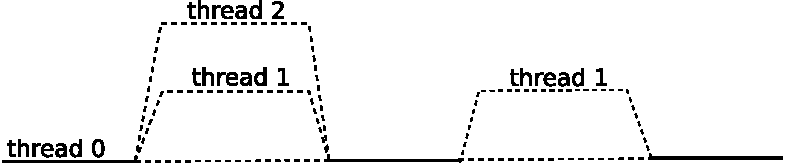
\includegraphics[width=0.9\linewidth]{fork_and_join}
  \end{center}
  \bigskip
  
\item Declaring parallel sections in the code is done using \textbf{OpenMP directives}

\item Specific \textbf{memory model} (shared / private variables)
\end{itemize}
\end{frame}

%%%%%%%%%%%%%%%%%%%%%%%%%%%%%%%%%%%%%%%%%%%%%%%%%%%%%%%%%%%%%%%%%%%%%%%
\begin{frame}
  \frametitle{Using OpenMP}
  
\begin{itemize}
\item \textbf{Compile-time} directives ({\tt \#pragma} in C)
  \begin{itemize}
  \item Interpreted by OpenMP-aware the compiler
  \item \alert{Silently} ignored otherwise
  \item Tell the compiler to generate parallel code
  \item \texttt{gcc}: \texttt{-fopenmp} option
  \end{itemize}

\medskip
  
\item Must \textbf{link} against OpenMP run-time library
  \begin{itemize}
  \item \texttt{gcc}: \texttt{-fopenmp} option
  \end{itemize}

\medskip
  
\item At \textbf{run-time}: \alert{environment variables} allow some control over OpenMP
\end{itemize}
\end{frame}

%%%%%%%%%%%%%%%%%%%%%%%%%%%%%%%%%%%%%%%%%%%%%%%%%%%%%%%%%%%%%%%%%%%%%%

\begin{frame}[fragile=singleslide]
  \frametitle{OpenMP in One Slide}

    \begin{minted}{C}
// sequential prologue
#pragma omp parallel for
for (int i = 0 ; i < n ; i++) {
  /*
   * All the iterations of this loop can
   * be executed in parallel
   */
}
// sequential epilogue 
\end{minted}


\texttt{gcc \alert{-fopenmp} prog\_omp.c -o prog\_omp}

\medskip

\begin{itemize}
\item ``normal'' sequential program until \texttt{\#pragma omp}
\item A \textbf{team of threads} is created
\item The iterations of the loop are \textbf{distributed} between them
\item \textbf{Barrier} at the end of the loop
\item ``normal'' sequential program then
\end{itemize}
\end{frame}



%%%%%%%%%%%%%%%%%%%%%%%%%%%%%%%%%%%%%%%%%%%%%%%%%%%%%%%%%%%%%%%%%%%%%%%
\begin{frame}[fragile=singleslide]
  \frametitle{Conditional Compilation and Run-Time OpenMP Functions}

\begin{block}{Conditional compilation}
\begin{minted}{C}
#ifdef _OPENMP
    // Code included only if the compiler supports OpenMP
    // With gcc, only if the -fopenmp option has been given
#endif
\end{minted}
\end{block}


\begin{block}{OpenMP run-time functions}
  With \mintinline{C}{#include <omp.h>}

\begin{itemize}
\item Enable a SPMD style of programming (as in MPI)
\item \mintinline{C}{omp_get_num_threads()}
\item \mintinline{C}{omp_get_thread_num()}
\item \mintinline{C}{omp_set_num_threads()}
\item ...
\end{itemize}
\end{block}

\end{frame}



%%%%%%%%%%%%%%%%%%%%%%%%%%%%%%%%%%%%%%%%%%%%%%%%%%%%%%%%%%%%%%%%%%%%%%%
\begin{frame}[fragile=singleslide]
  \frametitle{Hello world}

\small

\begin{columns}[t]
  \column{6cm}
  
\begin{block}{Programme}
\begin{minted}{C}
#ifdef _OPENMP
#include <omp.h>
#endif

int main()
{
  #pragma omp parallel 
  {
    #ifdef _OPENMP
    printf("Hello world, thread %d/%d\n",
          omp_get_thread_num(),
          omp_get_num_threads());
    #else 
    printf("Hello world\n");    
    #endif
  }
}
\end{minted}
\end{block}

\column{4cm}

\begin{block}{Exécution}
\scriptsize
\begin{verbatim} 
$ gcc hello.c -o hello
$ ./hello
Hello world
$ gcc -fopenmp hello.c \
 -o hello
$ export OMP_NUM_THREADS=4
$ ./hello
Hello world, thread 0/4
Hello world, thread 3/4
Hello world, thread 1/4
Hello world, thread 2/4
\end{verbatim}
\end{block}  
\end{columns}

\end{frame}



%%%%%%%%%%%%%%%%%%%%%%%%%%%%%%%%%%%%%%%%%%%%%%%%%%%%%%%%%%%%%%%%%%%%%%%
\begin{frame}
  \frametitle{OpenMP Directives}

\begin{framed}
  {\tt \#pragma omp} {\it directive [clause[[, ]clause]...]}   
\end{framed}
 
\textbf{Barrier} (synchronization) at the end by default 

\medskip

\begin{block}{Using directives}
\begin{itemize}
\item Jumping out of a parallel section is forbidden (\sout{goto}, \sout{setjmp/longjmp}, ...)
\item One directive per \texttt{\#pragma omp}
\item Case-sensitive

\item Directives $\subseteq$ $\{$ {\tt parallel, for, sections, section, single, master, critical,
  barrier, atomic, flush, ordered, threadprivate, ...} $\}$
\end{itemize}
\end{block}

\end{frame}




%%%%%%%%%%%%%%%%%%%%%%%%%%%%%%%%%%%%%%%%%%%%%%%%%%%%%%%%%%%%%%%%%%%%%%%
\begin{frame}
  \frametitle{OpenMP Memory Model}

  \begin{block}{Reminder}
    \textbf{Variable} : \alert{identifier} denoting a \alert{memory address}
  \end{block}
  
  \begin{columns}[t]
    \column{0.5\textwidth}

    Variables present in the original sequential code can be declared as {\it shared}
    or {\it private}) with OpenMP.

    \medskip
    
    \begin{itemize}
    \item \textbf{Shared}: all threads access the memory address of the original variable 

    \item \textbf{Private}: each thread ``owns'' a \alert{copy} %%locale
      of the original variable (all located at different memory addresses)
    \end{itemize}
    
    \column{0.5\textwidth}
    \begin{center}
      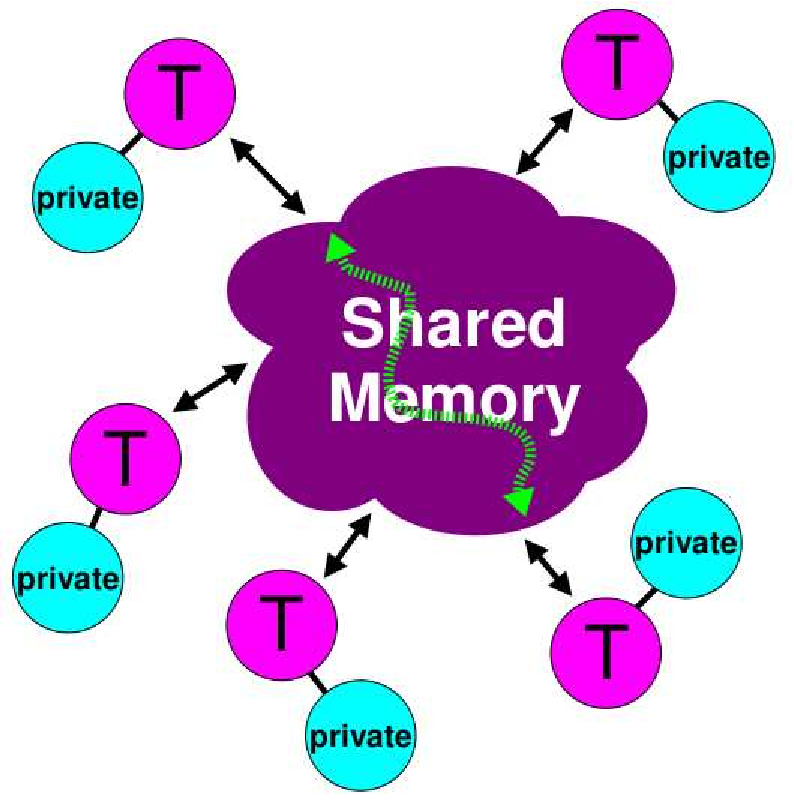
\includegraphics[width=\textwidth]{modele_mem_OpenMP}    

      {\tiny (after {\it An Overview of OpenMP 3.0}, R. van der Pas)} 
    \end{center}
  \end{columns}


\end{frame}



%%%%%%%%%%%%%%%%%%%%%%%%%%%%%%%%%%%%%%%%%%%%%%%%%%%%%%%%%%%%%%%%%%%%%%%
\begin{frame}
  \frametitle{OpenMP Memory Model (continued)}

  \begin{itemize}

  \item Variables declared \textbf{before} a parallel region are
    \textbf{shared by default}

      \medskip
      
    \item Their status can be modified using \alert{clauses} in OpenMP directives
      \begin{itemize}
      \item {\tt private, shared, firstprivate, lastprivate, default(shared),
          default(none), reduction, copyin}
      \end{itemize}

      \medskip
      
    \item Local variables of each thread are private (cf. infra)
      
    \end{itemize}  
\end{frame}



%%%%%%%%%%%%%%%%%%%%%%%%%%%%%%%%%%%%%%%%%%%%%%%%%%%%%%%%%%%%%%%%%%%%%%%
\begin{frame}
  \frametitle{\texttt{parallel} Directive}

\begin{framed}
  {\tt \#pragma omp parallel } {\it  [clause[[, ]clause]...]} \\
  {\it structured block} 
\end{framed}

\begin{itemize}
\item Create a \alert{thread team} (creation/recycling)   
\item \textbf{All} threads run the \textit{structured block}.
\end{itemize}

\begin{block}{Associated clauses}

\begin{itemize}
\item {\tt if(cond)}: {\tt cond == False} $\rightarrow$ no threads
  \begin{itemize}
  \item E.g., don't use all the machine for small problem
  \end{itemize}
  
\item  {\tt private} ({\it var\_list}), {\tt firstprivate} ({\it var\_list})

\mynote{{\tt copyin} uniquement pour les variables déclarées comme
  {\tt threadprivate} (voir plus loin)}

\item {\tt reduction} (cf. infra)
  
\item  {\tt num\_threads}({\it int}): force the size of the thread team

\end{itemize} 
\end{block}
\end{frame}
 


%%%%%%%%%%%%%%%%%%%%%%%%%%%%%%%%%%%%%%%%%%%%%%%%%%%%%%%%%%%%%%%%%%%%%%%
\begin{frame}[fragile=singleslide]

\begin{minted}{C}
int main()
{
    ...
    initialization();
    #pragma omp parallel ...
    {
         parallel_computation();
    }
    post_processing();
}
\end{minted}

\begin{exampleblock}{How to choose the number of threads}
By decreasing order of priority:

\small
\begin{tabular}[ht]{|l@{~:~}l|}
\hline
Compile-time &   \#pragma omp parallel num\_threads(16) \\
\hline
Run-time &  {\it omp\_set\_num\_threads(4)} \\
\hline
Environment variable &  export OMP\_NUM\_THREADS=4 \\
\hline
\end{tabular}
\normalsize
\end{exampleblock}
\end{frame}



%%%%%%%%%%%%%%%%%%%%%%%%%%%%%%%%%%%%%%%%%%%%%%%%%%%%%%%%%%%%%%%%%%%%%%%
\begin{frame}[fragile=singleslide]
  \frametitle{Predefined Variables are Shared by Default}
  
  \begin{columns}[t]
  \column{5cm}
\begin{block}{Program}
\begin{minted}{C}
#include <omp.h>
#include <stdio.h>

int main()
{
  int c=0;

  #pragma omp parallel 
  {
    c++;
    printf("c=%d thread %d\n",
        c, omp_get_thread_num());
  }
}
\end{minted}
\end{block}
    
    
    \column{5cm}
\begin{block}{Execution}    
  \small

\begin{verbatim}
$ export OMP_NUM_THREADS=4
$ ./a.out
c=1 thread 3
c=2 thread 0
c=3 thread 1
c=4 thread 2
\end{verbatim}
\end{block}    
  \end{columns}
\end{frame}



%%%%%%%%%%%%%%%%%%%%%%%%%%%%%%%%%%%%%%%%%%%%%%%%%%%%%%%%%%%%%%%%%%%%%%%
\begin{frame}[fragile=singleslide]
  \frametitle{Beware of Conflicts!}
  
  \small
  \begin{columns}[t]
  \column{5cm}
\begin{block}{Program}
\begin{minted}{C}
#include <omp.h>
#include <stdio.h>

int main()
{
  int c = 0;

  #pragma omp parallel
  {  
    for (int i=0; i<100000; i++)
        c++;
    printf("c=%d thread %d\n", 
        c, omp_get_thread_num());
  }
}
\end{minted}
\end{block}
    
    
    \column{5cm}
\begin{block}{Execution}    
\begin{verbatim}
$ export OMP_NUM_THREADS=4
$ ./a.out
c=100000 thread 0
c=200000 thread 3
c=270620 thread 2
c=286162 thread 1
\end{verbatim}
\end{block}    
  \end{columns}
\normalsize
\end{frame}


%%%%%%%%%%%%%%%%%%%%%%%%%%%%%%%%%%%%%%%%%%%%%%%%%%%%%%%%%%%%%%%%%%%%%%%
\begin{frame}[fragile=singleslide]
  \frametitle{\texttt{private} Clause}

 \texttt{private} variable:
  \begin{itemize}
  \item Each thread owns a (private) local copy
  \item \alert{Not initialized}
  \end{itemize}

\medskip

BUG~:
\begin{columns}[t]
  \column{5cm}
  
\begin{block}{Program}
\begin{minted}{C}
int main()
{
  int a = 100;
  #pragma omp parallel private(a)
  {
   /* This "a" is not the same
      as before */
    a = a + 10;
    printf("a=%d\n", a);
  }
  printf("After a=%d\n", a);
}
\end{minted}
\end{block}

  
  \column{5cm}
\begin{block}{Execution}
\small
\begin{verbatim} 
$ export OMP_NUM_THREADS=4
$ ./a.out 
a=-1208433038
a=-22
a=-22
a=-22
Apres a=100
\end{verbatim}
\end{block}  
\end{columns}
\end{frame}




%%%%%%%%%%%%%%%%%%%%%%%%%%%%%%%%%%%%%%%%%%%%%%%%%%%%%%%%%%%%%%%%%%%%%%%
\begin{frame}[fragile=singleslide]
  \frametitle{\texttt{firstprivate} Clause}
  
   \texttt{firstprivate} Variables;
  \begin{itemize}
  \item Each thread owns a (private) local copy
  \item Initialized with the preexisting value
  \end{itemize}
  
  \begin{columns}[t]
  \column{5cm}
\begin{block}{Program}
\begin{minted}{C}
  int main()
  {
  int a = 100;
  #pragma omp parallel \
                firstprivate(a)
  {
    a = a + 10;         // idem...
    printf("a=%d\n", a);
  }
  printf("After a=%d\n", a);
}
\end{minted}
\end{block}
    
    
    \column{5cm}
\begin{block}{Execution}    
  \small
\begin{verbatim}
$ export OMP_NUM_THREADS=4
$ ./a.out 
a=110
a=110
a=110
a=110
Apres a=100
\end{verbatim}
\end{block}    
  \end{columns}
\end{frame}

%%%%%%%%%%%%%%%%%%%%%%%%%%%%%%%%%%%%%%%%%%%%%%%%%%%%%%%%%%%%%%%%%%%%%%%

\begin{frame}[fragile=singleslide]
  \frametitle{Local Variables}

  \begin{itemize}
  \item All local variables in functions called from a parallel section are
        owned by the corresponding thread (on their stacks)

  \item Same goes for local variables declared inside the \textit{structured block}
  \end{itemize}

\small
\begin{columns}[t]
  \column[T]{5cm}
\begin{block}{Program}
\begin{minted}{C}
void func()
{
  int a = 10;
  a += omp_get_thread_num();
  printf("a=%d\n", a);
}

int main()
{
  #pragma omp parallel 
  func();
}
\end{minted}
\end{block}

\column[T]{5cm}
\begin{block}{Execution}
\begin{verbatim}
$ export OMP_NUM_THREADS=4
$ test2
10
11
12
13
\end{verbatim}
\end{block}
\end{columns}
\end{frame}

%%%%%%%%%%%%%%%%%%%%%%%%%%%%%%%%%%%%%%%%%%%%%%%%%%%%%%%%%%%%%%%%%%%%%%%

\begin{frame}[fragile=singleslide]
  \frametitle{Local Variables: My Opinion}


  \begin{columns}[t]
  \column[T]{6cm}
  \begin{alertblock}{Complex (avoid)}
    \begin{minted}{C}
int main()
{
  int a;
  #pragma omp parallel private(a)
  {
    a = ...;
    ...
  }
}

/**************************************/

int main()
{
  int a;
  #pragma omp parallel firstprivate(a)
  {

    ... a ...
  }
}

\end{minted}
\end{alertblock}

  \column[T]{4cm}
  \begin{exampleblock}{Simple (better)}
    \begin{minted}{C}
int main()
{
  
  #pragma omp parallel
  {
    int a = ...;
    ...
  }
}

/*************************/

int main()
{
  
  #pragma omp parallel
  {
    int b = a;
    ... b ...
  }
}
\end{minted}
\end{exampleblock}
\end{columns}

\end{frame}

%%%%%%%%%%%%%%%%%%%%%%%%%%%%%%%%%%%%%%%%%%%%%%%%%%%%%%%%%%%%%%%%%%%%%%%
\begin{frame}[fragile=singleslide]
  \frametitle{Reminders / Details}
  
\begin{block}{\bf \texttt{\#pragma omp parallel}}
  \begin{itemize}
  \item A \alert{\textbf{thread team}} is created
  \item The \textbf{encountered thread} belongs to it (\textbf{master})
  \item All threads of the team execute the \textit{structured block}
  \item Identifiers (``ranks'') 0 (master), 1, 2, \dots, \#threads - 1
    \begin{itemize}
      \item \mintinline{C}{omp_get_num_threads(), omp_get_thread_num()}
    \end{itemize}
  \item \textbf{Barrier} at the end
  \item Encountering thread then resumes sequential execution
  \end{itemize}
\end{block}
\end{frame}

%%%%%%%%%%%%%%%%%%%%%%%%%%%%%%%%%%%%%%%%%%%%%%%%%%%%%%%%%%%%%%%%%%%%%%%

\begin{frame}
  \frametitle{\texttt{for} Directive}
  
\begin{framed}
  {\tt \#pragma omp for } {\it  [clause[[, ]clause]...]}  \\
  {\it $\langle$ for loop $\rangle$} 
\end{framed}

\begin{alertblock}{\textbf{Worksharing} directive}
  Threads of the team cooperate and \textbf{divide} the work between them
\end{alertblock}

\medskip
  
Associated clauses~:
  \begin{itemize}
  \item  {\tt private} ({\it variable\_list}), {\tt firstprivate} ({\it variable\_list}), {\tt lastprivate} ({\it variable\_list})
  \item {\tt reduction}({\it operator: variable\_list})
  \item {\tt ordered}
  \item {\tt collapse}({\it n})
  \item {\tt  schedule}({\it type}, {\it taille})
  \item {\tt nowait}
  \end{itemize}
  
\end{frame}


%%%%%%%%%%%%%%%%%%%%%%%%%%%%%%%%%%%%%%%%%%%%%%%%%%%%%%%%%%%%%%%%%%%%%%%
\begin{frame}
  \frametitle{\texttt{for} Directive (continued)}

  \begin{block}{Canonical loop form}
  
 \centerline{ {\tt for (} {\it init\_expr} {\tt ; } {\it cond} {\tt ;} {\it increment})}
 
\begin{itemize}
\item Integer iteration variable

\item Loop counter updated with \texttt{++, --, +=, -=, var=var+inc,
    var=inc+var, var=var-inc}, integer increment

\item Condition: \texttt{<, >, <=, >=}. Bound is a fixed expression

\item No early exit ({\tt break}, {\tt return}, {\tt exit})
\item \texttt{continue} is allowed
\end{itemize}
\end{block}

\medskip

Consequences of the \texttt{for} directive:
\begin{itemize}
\item Implicit barrier at the end of the loop (except if {\tt nowait})
\item No barrier at the beginning
\item \textbf{The iteration variable is private}
\end{itemize}

\end{frame}

%%%%%%%%%%%%%%%%%%%%%%%%%%%%%%%%%%%%%%%%%%%%%%%%%%%%%%%%%%%%%%%%%%%%%%%

\begin{frame}[fragile=singleslide]
  \frametitle{Example}
\begin{minted}[fontsize=\normalsize]{C}
int main()
{
  int t[100];
  #pragma omp parallel 
  {
    #pragma omp for  
    for (int i = 0; i < 100; i++)
      t[i] = i;
  }
}
\end{minted}

  With 4 threads, the first one may {\bf for instance} compute the $t[i]$ from 0 to 24,
  the second from 25 to 49, ...
\end{frame}

%%%%%%%%%%%%%%%%%%%%%%%%%%%%%%%%%%%%%%%%%%%%%%%%%%%%%%%%%%%%%%%%%%%%%%%

% \begin{frame}[fragile=singleslide]
%   \frametitle{\texttt{lastprivate} Variable}

%   \begin{itemize}
%   \item Each thread owns a local (private) copy 
%   \item \alert{Not initialized}
%   \item The value at the end of the \textbf{last} iteration ($N-1$)
%     is written in the preexisting variable at the end of the loop
%   \end{itemize}

%   \begin{columns}[t]
%   \column{5.5cm}
%   \begin{block}{Program}
% \begin{minted}{C}
% int a;
  
% #pragma omp parallel 
% #pragma omp for lastprivate(a)
% for(int i = 0; i < 4; i++) {
%   a = i * 10;
%   printf("PAR a=%d thread %d \n",
%            a, omp_get_thread_num());
% }
% printf("SEQ a=%d %d\n", a);
% \end{minted}
% \end{block}
  
%   \column{5cm}
  
%   \begin{block}{Execution}
%     \small
% \begin{verbatim}
% $ export OMP_NUM_THREADS=4
% $ ./a.out 
% PAR a=0 thread 0
% PAR a=10 thread 1
% PAR a=20 thread 2
% PAR a=30 thread 3
% SEQ a=30
% \end{verbatim}
%   \end{block}  
% \end{columns}
% \end{frame}


%%%%%%%%%%%%%%%%%%%%%%%%%%%%%%%%%%%%%%%%%%%%%%%%%%%%%%%%%%%%%%%%%%%%%%%
\begin{frame}[fragile=singleslide]
  \frametitle{Short Form for the \texttt{for} directive}
  
\begin{framed}
  {\tt \#pragma omp parallel for } {\it  [clause[[, ]clause]...]}  \\
  {\it for loop} 
\end{framed}

Admits all clauses of {\tt parallel} and {\tt for}, except {\tt nowait}.

\medskip

\begin{minted}{C}
#pragma omp parallel
#pragma omp for
for (int i = 0 ; i < n ; i++) {
   ....
}

#pragma omp parallel for
for (int i = 0 ; i < n ; i++) {
   ....
}
\end{minted}
\end{frame}

%%%%%%%%%%%%%%%%%%%%%%%%%%%%%%%%%

\begin{frame}[fragile=singleslide]
  \frametitle{The \texttt{reduction} Clause}

  \small
\begin{columns}[t]
  \column{6.25cm}
  \begin{block}{Programme}
    \begin{minted}{C}
int main()
{
  int a[4][4], s=0;
  for (int i = 0; i < 4; i++)
      for (int j = 0; j < 4; j++)
        a[i][j] = i * 4 + j;
  #pragma omp parallel for reduction(+:s)
  for (int i = 0 ; i < 4 ; i++) {
      for (int j = 0; j < 4; j++)
          s += a[i][j];
      printf("PAR=%d : i=%3d  s=%d\n",
           omp_get_thread_num(), i, s);
     }
  }
  printf("SEQ s=%d\n", s);
}
\end{minted}
\end{block}
  
  \column{4.5cm}
  
  \begin{block}{Execution}
\small
\begin{verbatim}
$ export OMP_NUM_THREADS=4
$ ./a.out 
PAR=0 : i=  0  s=6
PAR=1 : i=  1  s=22
PAR=2 : i=  2  s=38
PAR=3 : i=  3  s=54
SEQ s=120
\end{verbatim}
  \end{block}  
\end{columns}
\normalsize

\mynote{commencer par expliquer comment on a parallélisé la boucle
  externe de la double boucle (i.e. 'j' mis en private)}

\mynote{
{\bf La matrice contient : \\ 
 0  1  2  3 \\
 4  5  6  7 \\
 8  9 10 11 \\
12 13 14 15 \\
}}

\mynote{{\bf La clause reduction s'applique à une variable partagée
qui (d'après moi) sera ``traitée comme une variable privée (avec
  firstprivate) à chaque thread'' durant l'exécution de la région
  parallèle, sauf à la fin au moment de la réduction.}}
\end{frame}

%%%%%%%%%%%%%%%%%%%%%%%%%%%%%%%%%%%%%%%%%%%%%%%%%%%%%%%%%%%%%%%%%%%%%%

\begin{frame}[fragile=singleslide]
  \frametitle{The \texttt{reduction} Clause (continued)}

  \begin{itemize}
  \item Operators : \verb$+, -, * , &, |, ˆ, &&, ||, min, max$
  \item Can define your own
  \end{itemize}
  
  \medskip

  Authorized on \texttt{omp for}, \texttt{omp parallel}, \dots

  \medskip
  
\begin{minted}{C}
int main()
{
  int m = 0;
  #pragma omp parallel reduction(max:m)
  {
    int tid = omg_get_thread_num();
    m = f(tid);
  }
  ...
}
\end{minted}
\end{frame}

%%%%%%%%%%%%%%%%%%%%%%%%%%%%%%%%%%%%%%%%%%%%%%%%%%%%%%%%%%%%%%%%%%%%%%

\begin{frame}[fragile=singleslide]
  \frametitle{New Features in \texttt{reduction}}

  \begin{columns}[b]
    \begin{column}{.1\textwidth}
      
\includegraphics[width=\textwidth]{Content.png}
    \end{column}
    \begin{column}{.9\textwidth}
      \begin{itemize}
      \item \texttt{reduction} on  \emph{arrays}
      \item ... or array \emph{slices}
      \item Starting with OpenMP 4.5
        \begin{itemize}
        \item November 2015, \texttt{gcc} $\geq 6.1$
        \end{itemize}
      \end{itemize}
    \end{column}
  \end{columns}

\bigskip
  
\begin{minted}[fontsize=\small]{C}
double *A = malloc(n * sizeof(*A));
...
#pragma omp parallel reduction(+:A[0:n])
{
    // Each thread own its own copy of A[0:n]
    for (int i = 0; i < n; i++) {
       A[i]= ....
    }
    ....
}
// A[i] contains the sum of the 
// private A[i]'s of all threads
\end{minted} 
\end{frame}

%%%%%%%%%%%%%%%%%%%%%%%%%%%%%%%%%%%%%%%%%%%%%%%%%%%%%%%%%%%%%%%%%%%%%%%

\begin{frame}
  \frametitle{Load Balancing in Loops}
  
  \texttt{omp for} admits load-balancing clauses: \texttt{schedule} and \texttt{nowait}
  
  \bigskip
  
  \begin{itemize}
  \item \texttt{nowait} clause:
    
    Removes the automatic barrier at the end of the loop
  
    \bigskip
  \item \texttt{schedule(mode, chunk\_size)} clause:
      
    4 modes: \texttt{static, dynamic, guided, runtime}
  \end{itemize}
  
  \bigskip

  Implementation-dependent if not specified (static on gcc)
\end{frame}

%%%%%%%%%%%%%%%%%%%%%%%%%%%%%%%%%%%%%%%%%%%%%%%%%%%%%%%%%%%%%%%%%%%%%%%
\begin{frame}[fragile=singleslide]
   \frametitle{\texttt{schedule} Example}
   \small
  
\begin{minted}{C}
#define MAX 10
int main()
{
  int a[MAX];
  #pragma omp parallel
  {
      int imax = 0;
      int imin = MAX;
      #pragma omp for schedule(static)
      for (int i = 0; i < MAX; i++) {
          imin = (i < imin) ? i : imin;
          imax = (i > imax) ? i : imax;
          a[i] = 1;
          sleep(1); /* simulate computation */
          printf("%3d:%3d\n",omp_get_thread_num(), i);
      }
      printf("T%d imin=%d imax=%d\n", omp_get_thread_num(), imin, imax);
  }
}
\end{minted}
\end{frame}

%%%%%%%%%%%%%%%%%%%%%%%%%%%%%%%%%%%%%%%%%%%%%%%%%%%%%%%%%%%%%%%%%%%%%%%

\begin{frame}[fragile=singleslide]
  \frametitle{\texttt{static} and \texttt{dynamic} Clauses }

  \texttt{schedule(...)}

  \footnotesize

\begin{columns}[t]
  \column[T]{3cm}
  
%%   \begin{block}{Rien(comme ``static'' mais 
%%       pas tres interessant car depend de l'implementation donc pas
%%       présenté...} 
%% \begin{verbatim}
%%   2:  6
%%   3:  9
%%   1:  3
%%   0:  0
%%   2:  7
%%   1:  4
%%   0:  1
%%   2:  8
%%   1:  5
%%   0:  2
%% thread 0 imin=0 imax=2
%% thread 1 imin=3 imax=5
%% thread 3 imin=9 imax=9
%% thread 2 imin=6 imax=8
%% \end{verbatim}
%%   \end{block}

  \begin{block}{static}
\begin{verbatim}
  1:  3
  3:  8
  2:  6
  0:  0
  1:  4
  3:  9
  2:  7
  0:  1
  1:  5
  0:  2
T1 imin=3 imax=5
T0 imin=0 imax=2
T2 imin=6 imax=7
T3 imin=8 imax=9
\end{verbatim}
  \end{block}

  \column[T]{3cm}
  \begin{block}{static, 2}
\begin{verbatim}
  1:  2
  3:  6
  2:  4
  0:  0
  1:  3
  3:  7
  0:  1
  2:  5
  0:  8
  0:  9
T0 imin=0 imax=9
T1 imin=2 imax=3
T3 imin=6 imax=7
T2 imin=4 imax=5
\end{verbatim}
  \end{block}  


  \column[T]{3cm}
  \begin{block}{dynamic, 2}
\begin{verbatim} 
  1:  4
  0:  0
  2:  6
  3:  2
  1:  5
  2:  7
  0:  1
  3:  3
  1:  8
  1:  9
T1 imin=4 imax=9
T3 imin=2 imax=3
T2 imin=6 imax=7
T0 imin=0 imax=1
\end{verbatim}
  \end{block}  

\end{columns}
\end{frame}

%%%%%%%%%%%%%%%%%%%%%%%%%%%%%%%%%%%%%%%%%%%%%%%%%%%%%%%%%%%%%%%%%%%%%%%
\begin{frame}
  \frametitle{Schedule}

  \begin{itemize}
  \item \texttt{schedule(static)}: block distribution
    
  \item \texttt{schedule(static, n)}: block-cyclic distribution.
    \begin{itemize}
    \item block size \texttt{n}
    \end{itemize}

%%  \bigskip

  \item \texttt{schedule(dynamic, n)}: chunks of \texttt{n} iterations are affected to available threads
  ($n = 1$ by default).

%%  \bigskip

  \item \texttt{guided}: like \texttt{dynamic} but the chunk size is proportional to the number of remaining iterations 

%%  \bigskip

\item \texttt{auto}: the OpenMP runtime does its magic
  
  \item \texttt{runtime}: choice is deferred until runtime \\
    Example~: {\tt export OMP\_SCHEDULE="static,1"}
  \end{itemize}
\end{frame}

%%%%%%%%%%%%%%%%%%%%%%%%%%%%%%%%%%%%%%%%%%%%%%%%%%%%%%%%%%%%%%%%%%%%%%%

\begin{frame}
  \frametitle{\texttt{single} Directive}

\begin{framed}
  {\tt \#pragma omp single } {\it directive [clause[[, ]clause]...]}  \\
  {\it structured block} 
\end{framed}

\begin{block}{Goal}
  Sequential portion inside a parallel region, \textit{i.e.}
  a code chunk executed by a \textbf{single} thread

\begin{itemize}
\item It can by \textit{any} thread
  
\item Implicit barrier at the end of \texttt{single}

\item {\tt nowait} et {\tt copyprivate} are incompatible clauses

\mynote{{\bf copyprivate(a) : ``envoie'' à la fin la valeur de 'a' aux autres
  threads} (cf. slide $+2$) (clause disponible uniquement pour {\tt single})}

\end{itemize}
\end{block}

\medskip

Possible clauses:
\begin{itemize}
\item  {\tt private} ({\it variable\_list}), {\tt firstprivate} ({\it variable\_list}), {\tt copyprivate} ({\it variable\_list})
\item  {\tt nowait}
\end{itemize}

\end{frame}

%%%%%%%%%%%%%%%%%%%%%%%%%%%%%%%%%%%%%%%%%%%%%%%%%%%%%%%%%%%%%%%%%%%%%%%
\begin{frame}[fragile=singleslide]
  \frametitle{\texttt{single} Directive}

\begin{columns}[t]
  \column{6cm}
  \begin{block}{Program}
\begin{minted}{C}
int main()
{
  int a = 10; 
  #pragma omp parallel firstprivate(a) 
  {
    #pragma omp single
    a = 20;
   
    printf("thread %d a=%d\n",
        omp_get_thread_num(), a);
  }
}
\end{minted}
\end{block}
  
  \column{4.5cm}
  
  \begin{block}{Execution}
\footnotesize
\begin{verbatim}
$ export OMP_NUM_THREADS=4
$ ./a.out 
thread 0 a=20
thread 1 a=10
thread 3 a=10
thread 2 a=10
\end{verbatim} 
  \end{block}  
\end{columns}
\end{frame}

%%%%%%%%%%%%%%%%%%%%%%%%%%%%%%%%%%%%%%%%%%%%%%%%%%%%%%%%%%%%%%%%%%%%%%%

\begin{frame}
    \frametitle{{\tt master} Directive}

\begin{framed}
  {\tt \#pragma omp master }  \\
  {\it structured block} 
\end{framed}

\bigskip

\begin{itemize}
\item No clause

\item \alert{\textbf{No implicit barrier at the end}}

\item Only thread \#0 (master) runs the \textit{structured block}
\end{itemize}
  
\end{frame}

%%%%%%%%%%%%%%%%%%%%%%%%%%%%%%%%%%%%%%%%%%%%%%%%%%%%%%%%%%%%%%%%%%%%%%%

\begin{frame}
  \frametitle{Synchronizations in OpenMP}

Several options:
  \begin{itemize}
  \item Barriers
  \item \texttt{atomic} and \texttt{critical}
  \item Locks via OpenMP runtime functions (not covered): \\
    {\tt omp\_init\_lock()}\\
    {\tt omp\_\{set,test\}\_lock()}\\
    {\tt omp\_unset\_lock()}\\
    {\tt omp\_destroy\_lock()}\\
\mynote{Je privilégie {\tt atomic} et {\tt critical} par rapport aux
  verrous car je privilégie les pragmas OpenMP aux fonctions OpenMP.}
  \end{itemize}
\end{frame}


%%%%%%%%%%%%%%%%%%%%%%%%%%%%%%%%%%%%%%%%%%%%%%%%%%%%%%%%%%%%%%%%%%%%%%%
\begin{frame}[fragile=singleslide]
  \frametitle{\texttt{barrier} Directive } 

  \begin{framed}
    {\tt \#pragma barrier}
  \end{framed}
  
  \bigskip

  All threads must \emph{enter} the barrier before any of the threads continue
  execution beyond the barrier

  \bigskip
  
\begin{alertblock}{Problems with C syntax}

\begin{minted}[fontsize=\normalsize]{C}
if (n != 0) 
     #pragma omp barrier   // syntactically incorrect
\end{minted}

\bigskip
   
\begin{minted}[fontsize=\normalsize]{C}
if (n != 0) {
     #pragma omp barrier   // OK
} 
\end{minted}
\end{alertblock}

\end{frame}



%%%%%%%%%%%%%%%%%%%%%%%%%%%%%%%%%%%%%%%%%%%%%%%%%%%%%%%%%%%%%%%%%%%%%%%
\begin{frame}[fragile=singleslide]
  \frametitle{\texttt{atomic} Directive} 
  
  \begin{framed}
    {\tt \#pragma omp atomic [ read | write | update ]}\\
    {\it atomic-update}
  \end{framed}

  \medskip

  \begin{itemize}
  \item The \textit{atomic-update} is \alert{atomic} (cannot be interrupted)
  \item \textit{atomic-update} of the type:
    \begin{itemize}
    \item \mintinline{C}{v = x;} or \mintinline{C}{x = expr;}
    \item \mintinline{C}{x += expr;} or \mintinline{C}{x = x + expr;}
      \begin{itemize}
      \item Works with \verb@ +, *, -, /, &, &&, ^, |, ||, >>, << @
      \item \textit{expr} must not reference $x$. 
      \end{itemize}
    \end{itemize}
    
  \item Only reading/writing/updating $x$ is atomic.
  \item Evaluation of \textit{expr} is not
  \end{itemize}
\end{frame}

%%%%%%%%%%%%%%%%%%%%%%%%%%%%%%%%%%%%%%%%%%%%%%%%%%%%%%%%%%%%%%%%%%%%%%%
\begin{frame}[fragile=singleslide]
  \frametitle{}

  \small
  \begin{columns}[t]
  \column{5.75cm}
\begin{block}{Program}
\begin{minted}{C}
#include <omp.h>

int main()
{
  int c = 0;
  #pragma omp parallel
  {
    for (int i = 0; i < 100000; i++) { 
       #pragma omp atomic
       c++; 
    }
    printf("c=%d thread %d\n",
      c, omp_get_thread_num());
  }
}
\end{minted}
\end{block}
    
    
    \column{4.5cm}
\begin{block}{Execution}    
\footnotesize
\begin{verbatim}
$ export OMP_NUM_THREADS=4
$ ./a.out
c=100000 thread 0
c=294308 thread 2
c=394308 thread 3
c=400000 thread 1
\end{verbatim}
\end{block}    
  \end{columns}
\normalsize

\mynote{Faire référence au m\^eme exemple (sans {\tt \#pragma omp
    atomic}) du début du cours. }

\end{frame}




%%%%%%%%%%%%%%%%%%%%%%%%%%%%%%%%%%%%%%%%%%%%%%%%%%%%%%%%%%%%%%%%%%%%%%%
\begin{frame}[fragile=singleslide]
  \frametitle{Advanced \texttt{atomic} Directive}
  \framesubtitle{Since OpenMP 3.0 (2008)} 
  
  {\scriptsize 
    \begin{framed}
      {\tt \#pragma omp atomic \alert{capture}}\\ 
      \textit{structured block}
    \end{framed}
  }

  \begin{itemize}
  \item Capture = saving the previous value (``capture'') + update 
    
  \item With the \texttt{capture} clause, \textit{structured block} can be: 

\begin{center}
  \begin{columns}[t]
    \column{0.3\textwidth}
    \mintinline{C}{{v = x; x = expr;}}\\
    \mintinline{C}{{v = x; x += expr;}}\\
    \mintinline{C}{{x += expr; v = x;}}\\
    \mintinline{C}{{v = x; x = x + expr;}}\\
    \mintinline{C}{{v = x; x = expr + x;}}\\
    \mintinline{C}{{x = x + expr; v = x;}}\\
    \mintinline{C}{{x = expr + x; v = x;}}\\
    
    \column{0.3\textwidth}
      \mintinline{C}{{v = x; x++;}}\\
      \mintinline{C}{{v = x; ++x;}}\\
      \mintinline{C}{{++x; v = x;}}\\
      \mintinline{C}{{x++; v = x;}}\\
  \end{columns}
\end{center}

\end{itemize}    
\end{frame}

%%%%%%%%%%%%%%%%%%%%%%%%%%%%%%%%%%%%%%%%%%%%%%%%%%%%%%%%%%%%%%%%%%%%%%

\begin{frame}[fragile=singleslide]
  \frametitle{Ultra-Advanced \texttt{atomic} Directive}

  \begin{exampleblock}{``Compare-and-Swap''}
\vspace*{-2ex}
\begin{minted}[fontsize=\small]{C}
#pragma omp atomic compare
if (x == old) x = new; 
\end{minted}
  \end{exampleblock}

  \begin{block}{``Compare-and-Swap'' with capture}
\vspace*{-2ex}
\begin{minted}[fontsize=\small]{C}
#pragma omp atomic compare capture
{ if (x == old) { x = new; }; else { cap = x; } }
\end{minted}
  \end{block}
  
  \begin{alertblock}{``Compare-and-Swap'', most general form}
\vspace*{-2ex}
\begin{minted}[fontsize=\small]{C}
#pragma omp atomic compare capture 
{ ok = x==old; if (ok) { x = new; } else { cap = x; } }
\end{minted}
  \end{alertblock}

  \begin{itemize}
  \item All CPUs have \emph{hardware} support for this operation
  \item Requires \texttt{gcc 12.2} (August 2022)
  \end{itemize}
  
\end{frame}



%%%%%%%%%%%%%%%%%%%%%%%%%%%%%%%%%%%%%%%%%%%%%%%%%%%%%%%%%%%%%%%%%%%%%%%
\begin{frame}
  \frametitle{\texttt{critical} Directive} 

\begin{framed}
  {\tt \#pragma omp critical } {\it [name]}  \\
  {\it structured block} 
\end{framed}

\bigskip

\begin{itemize}
\item Only a single thread may enter the \textit{structured block} simultaneously

\item ``\textbf{critical section}''
    
\item An incoming thread has to wait while another thread executes the \textit{structured block}
  
\item The \textit{name} allows to distinguish distinct critical sections.
\end{itemize}
\end{frame}



%%%%%%%%%%%%%%%%%%%%%%%%%%%%%%%%%%%%%%%%%%%%%%%%%%%%%%%%%%%%%%%%%%%%%%%
\begin{frame}[fragile=singleslide]
  \frametitle{Example of \texttt{critical} Directive }
  \framesubtitle{Adding an Item to a Linked List}

\begin{minted}{C}
struct item_t {
  int val;
  struct item_t *next;
};
...
struct item_t *list = (struct item_t *) malloc(sizeof(*list)); 
...
#pragma omp parallel 
{ 
   ...
   (struct item_t *) new =  malloc(sizeof(*nouv));
   new->val = ...
   #pragma omp critical 
   {
      new->next = list;
      list = new;
   }
   ...
}
\end{minted}

Exercise: do it with \texttt{atomic compare}
  
\end{frame}


%%%%%%%%%%%%%%%%%%%%%%%%%%%%%%%%%%%%%%%%%%%%%%%%%%%%%%%%%%%%%%%%%%%%%%%
\begin{frame}[fragile=singleslide]
  \frametitle{Differences Between \texttt{atomic} and \texttt{critical}}

\begin{description}

\item[\texttt{atomic}:]
  \begin{itemize}
    \item Intended to update variables
    \item Depends on hardware support
      \begin{itemize}
      \item ``Atomic'' CPU instructions (compare-and-swap or ll/sc)
    \item Implemented with locks as a last resort
    \end{itemize}
  \item Lighter overhead \textit{a priori}
  \item \alert{To be preferred if possible}
  \end{itemize}

\bigskip

\item[\texttt{critical}:]
  \begin{itemize}
    \item Intended to encompass a larger portion of code
    \item Implemented using locks
    \item Heavier overhead
  \end{itemize}

\end{description}
\end{frame}

%%%%%%%%%%%%%%%%%%%%%%%%%%%%%%%%%%%%%%%%%%%%%%%%%%%%%%%%%%%%%%%%%%%%%%%

\begin{frame}[label=golden_rule]
%  \frametitle{}

  \begin{center}
    \Huge \bf \alert{Golden rule of \\ multi-thread programming }
  \end{center}

  \bigskip
  
  {\Large \textbf{ALL} potentially conflicting accesses${}^*$
    to \textbf{shared} variables \alert{\textbf{MUST}} be protected (\texttt{atomic},
    \texttt{critical}, ...).}

  \bigskip

  $*$ at least one of them is a write
\end{frame}





%%%%%%%%%%%%%%%%%%%%%%%%%%%%%%%%%%%%%%%%%%%%%%%%%%%%%%%%%%%%%%%%%%%%%%% 
% \begin{frame}
%     \frametitle{Directive {\tt threadprivate}}

%     Permet de définir le statut des variables globales ou statiques
%     dans les threads (usage pas très fréquent).  

%   \bigskip

%     Une variable {\tt threadprivate} ne doit pas apparaître dans une autre
%     clause sauf pour {\tt copyin, copyprivate, schedule, num\_thread, if}.

%     \bigskip
    
%     Une variable  {\tt threadprivate} ne doit pas être une référence (C++).

% \end{frame}



% %%%%%%%%%%%%%%%%%%%%%%%%%%%%%%%%%%%%%%%%%%%%%%%%%%%%%%%%%%%%%%%%%%%%%%%
% \begin{frame}[fragile]
%   \frametitle{Directive {\tt threadprivate}}

% \small
% \begin{columns}[t]
%   \column{6.5cm}
%   \begin{block}{Programme}
% \begin{minted}{C}
% int a = 10;  // variable globale
% #pragma omp threadprivate(a)

% int main()
% {
%     #pragma omp parallel
%     {
%         int rang = omp_get_thread_num();
%         a += rang;
%         printf("thd=%d a=%d\n", rang, a);
%     }
%     printf("SEQ a=%d\n",a);
% }
% \end{minted}
% \end{block}
  
%   \column{4cm}
  
%   \begin{block}{Exécution}
% \begin{verbatim}
% $ export OMP_NUM_THREADS=4
% $ ./a.out 
% thd=0 a=10
% thd=3 a=13
% thd=1 a=11
% thd=2 a=12
% SEQ a=10
% \end{verbatim} 
%   \end{block}  
% \end{columns}
% \normalsize
  
% \mynote{{\tt copyin(a)} : la valeur de la variable 'a' de la région
%   séquentielle est transmise à tous les threads de la région parallèle.}

% \end{frame}



%%%%%%%%%%%%%%%%%%%%%%%%%%%%%%%%%%%%%%%%%%%%%%%%%%%%%%%%%%%%%%%%%%%%%%%
%%%%%%%%%%%%%%%%%%%%%%%%%%%%%%%%%%%%%%%%%%%%%%%%%%%%%%%%%%%%%%%%%%%%%%%
%%% Note sur flush :

% Uniquement besoin de flush pour rendre certaines variables ``visibles'' 
% entre les threads hors des points de synchronisation (points de
% synchronisation implicites (flush implicites) automatiquement placés 
% par OpenMP à l'entrée/sortie de certaines directives) 

% -> flush deconseillé par ``Using OpenMP'' (sauf pour les experts) : je
% préfère donc me limiter ici aux directives atomic/critical (voire aux
% locks) et ne pas les embrouiller/noyer avec les problemes de cohérence
% mémoire sur machine multi-processeurs (je garde ca pour CINAP) 

%%%%%%%%%%%%%%%%%%%%%%%%%%%%%%%%%%%%%%%%%%%%%%%%%%%%%%%%%%%%%%%%%%%%%%%
%%%%%%%%%%%%%%%%%%%%%%%%%%%%%%%%%%%%%%%%%%%%%%%%%%%%%%%%%%%%%%%%%%%%%%%



%%%%%%%%%%%%%%%%%%%%%%%%%%%%%%%%%%%%%%%%%%%%%%%%%%%%%%%%%%%%%%%%%%%%%%%
\begin{frame}
  \frametitle{Nested Parallelism}


  \begin{itemize}
\item A \texttt{parallel} directive inside a \texttt{parallel} directive

\medskip
  
\item In most cases, this is a no-op.
  \begin{itemize}
  \item No more ``available'' threads to work on the nested parallel region:
    they are all in the parent parallel region.
  \end{itemize}

  \medskip

\item It is possible to force the creation of a new thread teams (cf. spec)
  
\end{itemize}

\begin{alertblock}{My opinion}
  \begin{itemize}
  \item \textbf{STRICTLY USELESS} to do it voluntarily
  \item Could happen if a parallel program invoked a parallel library inside a parallel region
  \end{itemize}
\end{alertblock}
\end{frame}


%%%%%%%%%%%%%%%%%%%%%%%%%%%%%%%%%%%%%%%%%%%%%%%%%%%%%%%%%%%%%%%%%%%%%%%
% \begin{frame}[fragile]
%   \frametitle{Parallélisme imbriqué}

% \small
% \begin{columns}[t]
%   \column{6cm}
%   \begin{block}{Programme}
% \begin{minted}{C}
% #define MAX 4

% #pragma omp parallel for  
% for (int i = 0; i < MAX; i++) {
%     #pragma omp parallel for  
%     for (int j = 0; j < MAX; j++) {
%       printf("%3d:(%2d,%2d) \n",
%          omp_get_thread_num(), i, j);
%     }
% }
% \end{minted}
% \end{block}
  
%   \column{4cm}
  
%   \begin{block}{Exécution}
% {\scriptsize
% \begin{verbatim}
% $ export OMP_NUM_THREADS=4
% $ export OMP_NESTED=TRUE 
%   0:( 2, 0) 
%   2:( 2, 2) 
%   0:( 0, 0) 
%   3:( 2, 3) 
%   3:( 0, 3) 
%   3:( 1, 3) 
%   2:( 1, 2) 
%   0:( 1, 0) 
%   1:( 1, 1) 
%   1:( 2, 1) 
%   1:( 0, 1) 
%   2:( 0, 2) 
%   3:( 3, 3) 
%   0:( 3, 0) 
%   1:( 3, 1) 
%   2:( 3, 2) 
% \end{verbatim} 
% }
%   \end{block}  
% \end{columns}
% \normalsize


% \end{frame}


% \note{
% \begin{itemize}
% \item Combien de threads créés en tout avec nested ? 4 ? 16 ?
% Avec {\tt gcc -fopenmp} sur commodore : 6 threads supp créés donc 7 threads 
% en tout !!
% Pas clair, et comme l'exécution parallèle se déroule comme s'il y a
% avait 16 threads, leur dire pour l'instant que ``l'execution des 2
% régions est faite en parallele comme si 16 threads étaient utilisés''... 

% Remarque : possible de limiter le nombre de threads créés par OpenMP
% avec la variable d'environnement \texttt{OMP\_THREAD\_LIMIT} (la limite
% incluant le thread master et tous les threads supplémentaires créés
% par OpenMP ({\it helper threads})). 

% \item  Schéma : 

%   \includegraphics[scale=0.3]{nested} 

% \end{itemize}
% }


% \note{
%   Spec3.0 : ``If nested parallelism is disabled, or is not supported
%   by the OpenMP implementation, then the new team that is 
% created by a thread encountering a parallel construct inside a
% parallel region will consist only of the encountering thread.''

% Du coup, si OMP\_NESTED=FALSE, alors on a en sortie : 
% \begin{alltt}
% \$ export OMP\_NUM\_THREADS=4
% \$ export OMP\_NESTED=FALSE
%   0:( 0, 0) 
%   0:( 0, 1) 
%   0:( 0, 2) 
%   0:( 0, 3) 
%   0:( 3, 0) 
%   0:( 3, 1) 
%   0:( 3, 2) 
%   0:( 3, 3) 
%   0:( 1, 0) 
%   0:( 1, 1) 
%   0:( 1, 2) 
%   0:( 1, 3) 
%   0:( 2, 0) 
%   0:( 2, 1) 
%   0:( 2, 2) 
%   0:( 2, 3) 
% \end{alltt} 
% mais 3 threads supplémentaires sont bien créés dans la 1ere région
% parallèle : la deuxième région parallèle est elle exécutée en 
% séquentiel et chacun des 4 threads de la 1ere région y appara\^it
% comme le thread ``master'' donc avec le numéro 0.  
% }

% \note{D'apres tutorial IWOMP: danger de nested est juste de pas
%   controler le nombre de threads (et de surcharger les coeurs CPU),
%   surtout si on fait bcp de récursion avec.}




%%%%%%%%%%%%%%%%%%%%%%%%%%%%%%%%%%%%%%%%
\begin{frame}[fragile=singleslide]
  \frametitle{OpenMP Runtime Library}

Some common functions (with \mintinline{C}{#include <omp.h>}):
\begin{itemize}
  \item \mintinline{C}{void omp_set_num_threads(int num\thread)}: sets the number
    of threads to use in subsequent parallel regions
    
  \item mintinline{C}{\tt int omp\_get\_num\_threads(void)}: return the number of threads in the current team
  \item \mintinline{C}{int omp_get_max_threads(void)}: upper bound on \#threads in new teams
  \item \mintinline{C}{int omp_get_thread_num(void)}
  \item \mintinline{C}{int omp_get_num_procs(void)}
  \item \mintinline{C}{int omp_in_parallel(void)}: return true if we are inside a parallel region
  \item \mintinline{C}{double omp_get_wtime(void)}
\end{itemize}

  
\end{frame}


%%%%%%%%%%%%%%%%%%%%%%%%%%%%%%%%%%%%%%%%%%%%%%%%%%%%%%%%%%%%%%%%%%%%%%%
\begin{frame}
  \frametitle{Environment Variables}
  \begin{itemize}
  \item {\tt OMP\_NUM\_THREADS}
  \item {\tt OMP\_SCHEDULE} :

{\tt export OMP\_SCHEDULE="static,4"}

{\tt export OMP\_SCHEDULE="dynamic"}

%   \item {\tt OMP\_DYNAMIC} :
    
%     \begin{itemize}
%     \item affectée avec {\tt TRUE} le nombre de threads peut-être ajusté par
%       l'environnement d'exécution pour améliorer l'utilisation du système.
      
%     \item affectée avec {\tt FALSE} l'ajustement est désactivé.
      
%     \item la valeur par défaut est système-dépendant.
%     \end{itemize}

  \item ...
    
  \end{itemize}

  
\end{frame}


\begin{frame}[fragile=singleslide]
  \frametitle{Cheat Sheet}

  \begin{exampleblock}{Most common}
    \begin{itemize}
    \item The \textit{must} : \verb|#pragma omp parallel for|
    \item \verb|atomic|  \verb|critical| directives
    \item \verb|schedule| and \verb|reduction| clauses
    \end{itemize}
  \end{exampleblock}

  \begin{block}{Less common : SPMD mode}
    \begin{itemize}
    \item Parallel region with explicit \verb|#pragma omp for| inside
    \item \verb|omp_get_thread_num()| and \verb|omp_get_num_threads()|
    \item \verb|barrier| or \verb|single| directives
    \end{itemize}
  \end{block}

  \begin{alertblock}{Rare (reserved for the most delicate cases...)}
    Everything else!
  \end{alertblock}
\end{frame}

% %%%%%%%%%%%%%%%%%%%%%%%%%%%%%%%%%%%%%%%%%%%%%%%%%%%%%%%%%%%%%%

% \begin{frame}
%   \frametitle{Threads POSIX}

%   \begin{block}{Bibliothèque \texttt{pthread}}
%     \begin{itemize}
%     \item POSIX = Portable Operating System Interface for uniX
%     \item Threads POSIX = interface portable pour
%       \begin{itemize}
%       \item Créer des threads
%       \item Synchroniser des threads entre eux
%       \end{itemize}
%     \end{itemize}
%   \end{block}

%   \begin{alertblock}{Programmation \og bas-niveau\fg{}}
%     \begin{itemize}
%     \item Parallélisme explicite (et gestion \og manuelle\fg{})
%     \item Débugage potentiellement ardu
%     \end{itemize}
%   \end{alertblock}
% \end{frame}

% %%%%%%%%%%%%%%%%%%%%%%%%%%%%%%%%%%%%%%%%%%%%%%%%%%%%%%%%%%%%%

% \begin{frame}[fragile]
%   \frametitle{Threads POSIX (suite)}

%   \begin{exampleblock}{Modèle \og \textit{fork/join}}
% \begin{minted}{C}
% #include <pthread.h>
% int pthread_create(pthread_t *thread, const pthread_attr_t *attr,
%                             void *(*start_routine) (void *), void *arg);
% int pthread_join(pthread_t thread, void **retval);
% \end{minted}
%   \end{exampleblock}

%   \begin{block}{Gestion de la mémoire}
%     \begin{itemize}
%     \item Tout l'espace du processus accessible à tous les threads
%     \item Variables \og privées\fg{} (sur la pile de chaque thread)
%     \item Variables globales $\rightarrow$ partagées
%     \item Variables sur le tas $\rightarrow$ partagées (si adresse connue)
%     \end{itemize}
%   \end{block}
  
% \end{frame}
%%%%%%%%%%%%%%%%%%%%%%%%%%%%%%%%%%%%%%%%%%%%%%%%%%%%%%%%%%%%%% 

\begin{frame}
  \frametitle{Tâches OpenMP (depuis v3.0, 2008)}

  \begin{alertblock}{Point d'orthographe}
  \begin{description}
    \item[Tache] marque, salissure, souillure. \textit{Une tache d'encre}
    \item[Tâche] travail à exécuter. \textit{Une tâche ardue}
    \end{description}
  \end{alertblock}

  \pause
  
  \begin{block}{``Rappel'' : \bf \texttt{\#pragma omp parallel}}
    \begin{itemize}
    \item Une \alert{\textbf{équipe de threads}} est crée
    \item ...
    \item Une \alert{\textbf{tâche implicite}} est créée pour chaque thread
    \item Elle lui est \textbf{liée} (peut pas migrer sur un autre thread)
    \end{itemize}
  \end{block}
  
  \medskip
  
  \textbf{tâche} = code + données associées, le tout exécuté par un thread
\end{frame}

%%%%%%%%%%%%%%%%%%%%%%%%%%%%%%%%%%%%%%%%%%%%%%%%%%%%%%%%%

\begin{frame}
  \frametitle{Directive \texttt{omp task}}

  \begin{framed}
  {\tt \#pragma omp task } {\it [clause], [clause], ...}  \\
  {\it bloc structuré} 
\end{framed}

\begin{itemize}
\item Le thread qui rencontre ceci crée une \textbf{tâche explicite}
\item Exécution \alert{immédiate} ou \alert{différée}
\item Exécution par un des threads de l'équipe... si disponible
\pause
\item Un thread peut suspendre l'exécution d'une tâche et en démarrer/reprendre
  une autre...
  \item ... Mais seulement lors d'un \emph{task scheduling points}
\end{itemize}
\end{frame}

%%%%%%%%%%%%%%%%%%%%%%%%%%%%%%%%%%%%%%%%%%%%%%%%%%%%%%%%%%%

\begin{frame}
  \frametitle{``Task Pool''}

  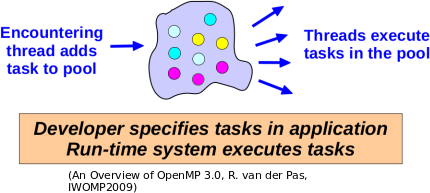
\includegraphics[width=\textwidth]{omp_task_pool.png}
\end{frame}


%%%%%%%%%%%%%%%%%%%%%%%%%%%%%%%%%%%%%%%%%%%%%%%%%%%%%%%%%%% 

\begin{frame}
  \frametitle{Synchronisation des tâches}
  \framesubtitle{Modèle \emph{Fork/Join}}
  

  \begin{block}{Barrières ``normales''}
    \begin{itemize}
    \item Implicites : à la fin d'une région parallèle, de \texttt{omp for}, ...
    \item Explicites : \texttt{\bf \#pragma omp barrier}
    \end{itemize}

    \medskip
    
    \textbf{Garantie} : Toutes les tâches crées par un thread de l'équipe courante sont
    terminées à la sortie de la barrière
  \end{block}
  
  \bigskip
  
  \begin{exampleblock}{Barrière de tâches : \texttt{\bf \#pragma omp taskwait}}
    \begin{itemize}
    \item La tâche courante attend la terminaison de ses tâches \alert{filles}
    \item Seulement filles directes, pas descendantes
    \end{itemize}
  \end{exampleblock}  
\end{frame}

%%%%%%%%%%%%%%%%%%%%%%%%%%%%%%%%%%%%%%%%%%%%%%%%%%%%%%%%%%%%%%

\begin{frame}[fragile]
  \frametitle{Exemple : parcours d'une liste chainée}

\begin{minted}[fontsize=\small]{C}
struct item_t {
  void * data;
  struct item_t * next;
};
struct item_t * head;
\end{minted}

\begin{columns}[T]
  \begin{column}{0.49\textwidth}
    \begin{block}{Séquentiel}
\begin{minted}[fontsize=\small,stripnl=false]{C}
struct item_t * e = head;


while (e != NULL) {

  process(e->data);
  e = e->next;
}
\end{minted}
    \end{block}
  \end{column}

  \begin{column}{0.49\textwidth}
    \begin{block}{Avec tâches\phantom{Sq}}
\begin{minted}[fontsize=\small]{C}
struct item_t * e = head;
#pragma omp parallel
#pragma omp single
while (e != NULL) {
  #pragma omp task
  process(e->data);
  e = e->next;
}
\end{minted}
    \end{block}
  \end{column}
\end{columns}
\end{frame}

\begin{frame}[fragile]
  \frametitle{Exemple : descente dans un arbre binaire}

\begin{minted}{C}
struct tree_t {
  ...
  struct tree_t *left, *right;
};
struct tree_t *root;
\end{minted}

\begin{columns}[T]
  \begin{column}{0.49\textwidth}
    \begin{block}{Séquentiel}
\begin{minted}[stripnl=false]{C}
void parcours(struct tree_t *t)
{
  ...
  if (t->left) 

      parcours(t->left);
  if (t->right) 

      parcours(t->right);
}


parcours(root);
\end{minted}
    \end{block}
  \end{column}

  \begin{column}{0.49\textwidth}
    \begin{block}{Avec tâches\phantom{Sq}}
\begin{minted}{C}
void parcours(struct tree_t *t)
{
  ...
  if (t->left) 
      #pragma omp task
      parcours(t->left);
  if (t->right) 
      #pragma omp task
      parcours(t->right);
}
#pragma omp parallel
#pragma omp single
parcours(root);
\end{minted}
    \end{block}
  \end{column}
\end{columns}
\end{frame}

%%%%%%%%%%%%%%%%%%%%%%%%%%%%%%%%%%%%%%%%%%%%%%%%%%%%%%%%%%%%%%%

\begin{frame}
  \frametitle{Directive \texttt{omp task}}

  \begin{framed}
  {\tt \#pragma omp task } {\it [clause], [clause], ...}  \\
  {\it bloc structuré} 
\end{framed}

\medskip

Clauses associées :
  \begin{itemize}
  \item  {\tt private} ({\it variable\_list}), {\tt firstprivate} ({\it
      variable\_list}), {\tt shared} ({\it variable\_list})
  \item {\tt default(shared | none)}
  \item {\tt untied}
  \item {\tt depend}({\it dependance-type}: {\it list})
  \item {\tt if({\it expression})}
  \end{itemize}  
\end{frame}

%%%%%%%%%%%%%%%%%%%%%%%%%%%%%%%%%%%%%%%%%%%%%%%%%%%%%%%%

\begin{frame}[fragile]
  \frametitle{Tâches : portée des variables}

  \begin{itemize}
  \item Le plus utile avec les tâches : \textbf{firstprivate}
  \item Attribut \textbf{firstprivate} par défaut sur toutes les variables...
  \item  \alert{\bf sauf} si elles sont déjà considérées comme \textbf{shared}
    \begin{itemize}
    \item Variable globale
    \item Variable déclarée avant la région parallèle
    \item Variable explicitement marquée comme \texttt{shared}
    \end{itemize}
  \end{itemize}

  \begin{alertblock}{\bf Attention aux variables partagées sur la pile}
\begin{minted}{C}
void f()
{
    int i = 3;
    #pragma omp task shared(i)
    printf("%d\n", i);
}

#pragma omp parallel
#pragma omp single
f();
\end{minted}
  \end{alertblock}
\end{frame}

%%%%%%%%%%%%%%%%%%%%%%%%%%%%%%%%%%%%%%%%%%%%%%%%%%%%%%%

\begin{frame}[fragile]
  \frametitle{Tâches : cas où \texttt{shared} est a priori nécessaire}

\begin{minted}{C}
struct tree_t {
  ...
  struct tree_t *left, *right;
};
struct tree_t *root;

/* Renvoie le nombre de noeuds de l'arbre. */
int size(struct tree_t *t)
{
  int s_left = 0, s_right = 0;
  if (t->left)
      #pragma omp task shared(s_left)
      s_left = size(t->left);
  if (t->right) 
      #pragma omp task shared(s_right)
      s_right = size(t->right);
  #pragma omp taskwait
  return 1 + s_left + s_right;
}
#pragma omp parallel
#pragma omp single
printf("%d\n", size(root));
\end{minted}
\end{frame}

%%%%%%%%%%%%%%%%%%%%%%%%%%%%%%%%%%%%%%%%%%%%%%%%%%%%%%%

% \begin{frame}
%   \frametitle{Tâches : ordonnancement}

%   \begin{block}{Liaison tâche $\leftrightarrow$ thread}
%     \begin{itemize}
%     \item Par défaut les tâches sont \textbf{tied} (liées)
%     \item[$\rightarrow$] toujours exécutées par le même thread (celui qui les a crées)
%     \item Tâche suspsendue seulement aux \emph{task scheduling points} :
%       création/terminaison de tâche, barrière, \texttt{taskwait}, \texttt{taskyield}
%     \end{itemize}
%   \end{block}

%   Problème potentiel : déséquilibrage de charge

%   \begin{exampleblock}{Clause \textbf{untied}}
%     \begin{itemize}
%     \item La tâche peut passer d'un thread à l'autre lors d'un \emph{task scheduling point}
%     \item \alert{Attention aux variables \texttt{threadprivate}}
%     \item \alert{Attention à l'indice du thread}
%     \item \alert{Attention aux sections critiques}
%     \end{itemize}
%   \end{exampleblock}  
% \end{frame}

%%%%%%%%%%%%%%%%%%%%%%%%%%%%%%%%%%%%%%%%%%%%%%%%%%%%%%%%%%%

\begin{frame}[fragile]
  \frametitle{Tâches : granularité}

  \textbf{Créer une tâche a un coût non-trivial}

  \bigskip

  \begin{exampleblock}{Ne pas créer des tâches minuscules}
    \begin{itemize}
    \item \emph{Clause} \textbf{if} de la directive \texttt{omp task}
      \begin{itemize}
      \item \texttt{\#pragma omp task if(prof < PROF\_MAX)}
      \item La tâche est \alert{quand même créée}...
      \item ...mais exécutée tout de suite par le thread courant
      \end{itemize}

      \medskip

    \item \emph{Instruction} \texttt{if}:
\begin{minted}{C}
if (prof < PROF_MAX) {
  #pragma omp task
  stuff(...);
} else {
  stuff(...);
}
\end{minted}
      \item[$\rightarrow$] à privilégier a priori
    \end{itemize}
  \end{exampleblock}
  
\end{frame}

%%%%%%%%%%%%%%%%%%%%%%%%%%%%%%%%%%%%%%%%%%%%%%%%%%%%%%%%

\begin{frame}
  \frametitle{Tâches : dépendances}

  TODO...
\end{frame}

%%%%%%%%%%%%%%%%%%%%%%%%%%%%%%%%%%%%%%%%%%%%%%%%%%%%%%%%

\begin{frame}
  \frametitle{Tâches : dépendances}
  \framesubtitle{Exemple de la mort (Christian Terboven)}
  
  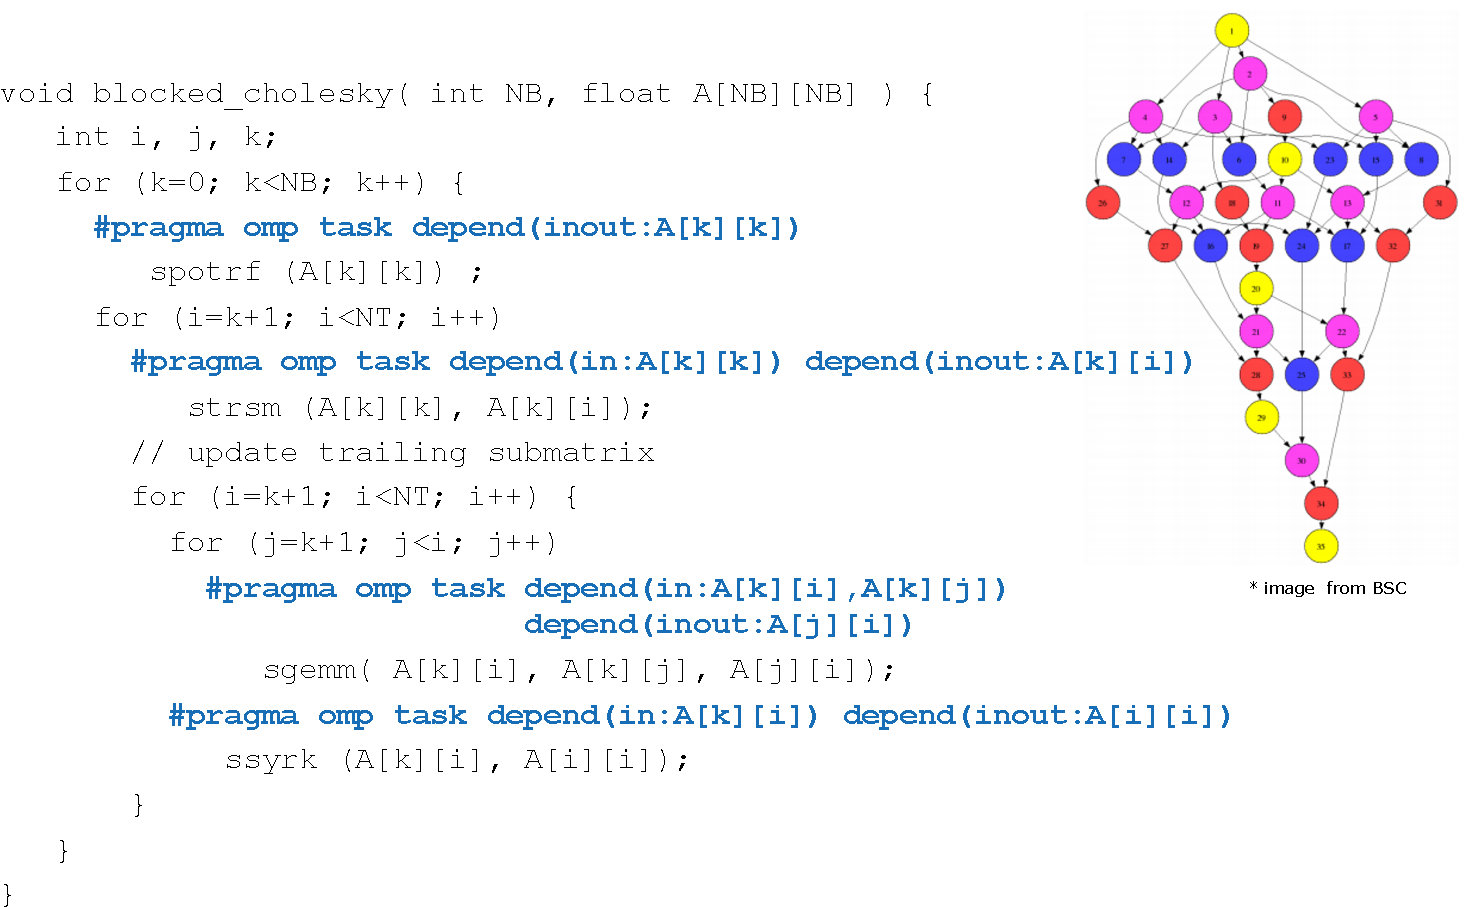
\includegraphics[width=\textwidth]{block_cholesky_tasking}
  
\end{frame}


\end{document}

%%% Local Variables:
%%% TeX-command-extra-options: "-shell-escape"
%%% TeX-engine: xetex
%%% End: